%!TEX root = mainfile.tex

\subsection{James Webb Space Telescope} % (fold)
\label{sub:james_webb_space_telescope}
	The James Webb Space Telescope (JWST) is a near-infrared space based telescope. Formerly known as the Next Generation Space Telescope, it was renamed after the NASA administrator James Edwin Webb in 2002. It is an international collaboration between NASA, the European Space Agency (ESA) and the Canadian Space Agency (CSA). The JWST’s capabilities will enable a broad range of investigations across many different fields in astronomy. However, its primary goal is to observe the most distant objects in our universe that are beyond the reach of any current ground or spaced based instruments. More importantly for our specific goals it will enable the study of the epoch of re-ionisation and the first stars\cite{jwst_nasa}.

	The JWST consists of four main instrument components:
	\begin{itemize}
		\item Near-Infrared Camera (NIRCam),
		\item Near-Infrared Spectrograph (NIRSpec),
		\item Mid-Infrared Instrument,
		\item Fine Guidance Sensor.
	\end{itemize}

	NIRCam uses a technique of CCD photometry to measure the magnitude of high redshift galaxies. It consists of ten mercury-cadmium-telluride (HgCdTe) detector arrays which are analogous to CCD’s found in digital cameras. Coronagraphs enable NIRCam to collate images of very faint objects around a central bright object\cite{jwst_nasa}.

	NIRSpec enables the JWST to obtain the spectrums of high redshift galaxies. It is comprised of micro shutter array with \num{62000} shutters that can be closed and opened individually meaning that the JWST can record the spectrums of one hundred different objects simultaneously. The device will have a total field of view of $3\times3$ arcminutes. As well as the micro shutter array NIRSpec will also have five fixed slits for high constant spectroscopy. There is an integral field unit spectrograph (IFU) with thirty slicers meaning that the spectrums of extended bodies can be found. The wavelength range over which NIRSpec can successfully operate is \SI{0.6}{\micro\metre} to \SI{5}{\micro\metre}\cite{jwst_nasa}.

	The Mid-Infrared Instrument will be used to obtain the spectrums of objects similar to NIRSpec. However the range over which it will operate will be \SI{5}{\micro\metre} to \SI{29}{\micro\metre}\cite{jwst_nasa}.

	Fine Guidance sensor (FGS) is a sensitive camera that will provide critical information for the JWST’s altitude control system. Its main functions include obtaining images for target acquisition and providing guide stars for the alignment and phasing for the segments of the primary mirror\cite{stsci_edu}.

	The JWST’s primary advantage over other current (and planned) space telescopes is its large primary mirror which has a diameter of 6.5\,metres. The next largest mirror of any spaced based telescope belongs to the Hubble Space Telescope (HST) which has a diameter of 2.4\,metres. JWST’s primary mirror is fabricated from eighteen beryllium segments each with a diameter 1.3\,metres which when correctly phased together act as a single mirror. The mirror phasing is achieved due to the fact that every segment has six degrees of rotational freedom by way actuators attached to their underside and the back plane. The back plane holds the primary mirror structure together\cite[p.~568--569]{gardner2006james}.
	\begin{figure}[!htbp]
		\centering
			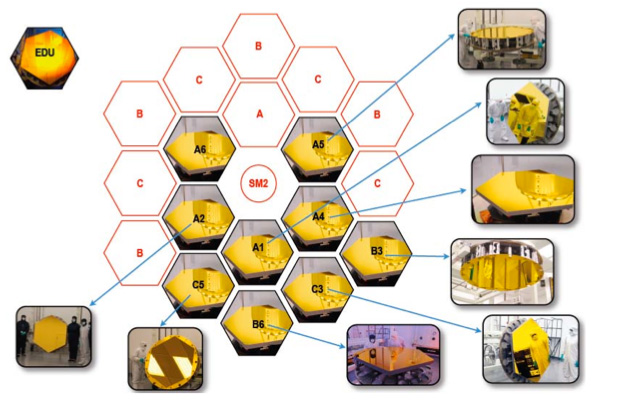
\includegraphics[width=0.6\textwidth]{../Images/JWST_mirror_construction.jpeg}
		\caption{\cite{primary_mirror_construction}\label{fig:james_web_layout}}
	\end{figure}

	The adjustability of JWST’s primary mirror allows for active optics, as discussed in Section~\ref{ssub:adaptive_optics}. When a mirror of this size pivots to look at different portions of space it naturally bends and deforms. By focusing on a reference object this deformity can be constantly corrected using the actuators connected to each segment of the primary mirror. It will be coated in gold to ensure a maximum reflectivity of 98\%\cite{mtwilson}.

	The Orbit of the JWST will lie at the second Lagrange point (L2) \SI{150000}{\kilo\metre} from Earth. L2 is one of five solutions to the three body problem posed by Joseph Louie Lagrange. It means that when the JWST is in orbit, the sun moon and earth will all stay in the same position relative to each other. The orbit is slightly inclined with respect to the elliptical plane, avoiding moon and earth eclipses of the sun, thus ensuring continuous electrical power is supplied. Orbit shown below in figure~\ref{fig:}\cite{primary_mirror_construction}.
	\begin{figure}[!htbp]
		\centering
			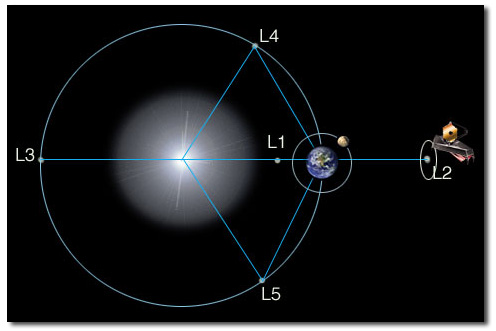
\includegraphics[width=0.5\textwidth]{../Images/JWST_orbit_L2.jpeg}
		\caption{\cite{jwst_orbit_l2}\label{fig:james_web_layout}}
	\end{figure}

	The JWST is fitted with a sunshield which reduces the incident radiation of approximately 200 KW to a few milliwatts. This solar attenuation is achieved through the five layer design of the sunshield. Each layer is separated from the next via a vacuum which allows for passive cooling of the JWST. The sunshield will a surface area of approximately \SI{250}{\square\metre} which is too large to fit inside any current spacecraft so will be unfolded into position once the JWST is in orbit at L2. Due to this size, solar radiation will cause a build-up of angular momentum throughout its service. This will be offset by firing service thrusters used primarily for obit maintenance.

	The JWST is a three mirror anastigmat meaning it can minimize the three main optical aberrations, namely; spherical aberration, coma and astigmatism. The effective focal length of the mirrors combined is \SI{131.4}{\metre}. The basic layout can be seen in Figure~\ref{fig:james_web_layout}.

	For the most part the JWST will be background limited as opposed to diffraction limited. The background is due mostly to scattered zodiacal light, scattered starlight and thermal emission from the sunshield. The background due to these factors can be seen in Table~\ref{tab:JW_exposure_times_for_galaxies}. The imaging performance of the JWST will be diffraction limited (i.e.\ limited by the optical power of the telescope) at \SI{2}{\micro\metre} with a Strehl ratio greater than 0.80.

	The field of view refers to the fraction of the celestial sphere that the telescope can point at any given moment. The main limitation to the JWST’s field of view is the sunshield means that only 31\% of the sky can be seen for more than 197\,days. All regions of sky have at least 51\,days of continuous visibility per year\cite[p.~561--572]{gardner2006james}.

	Table~\ref{tab:JW_exposure_times_for_galaxies} below shows the information required in order to calculate exposure times for galaxies of given red shifts and magnitudes at a set signal to noise ratio.
	\begin{table}[!htbp]
		\begin{center}
			\begin{tabular}{c|c}
				Read Noise 					& 10 \\
				Dark Current 				& \SI{0.018}{\electron\per\second\per\pixel} \\
				Diameter of Primary Mirror 	& \SI{8.2}{\metre} \\
				Quantum Efficiency 			& 0.8 \\
				Sky Background 				& 0.005\,photon s$^{-1}$pixel$^{-1}$) \\
				Gain 						& 1.8\si{e}ADU$^{-1}$) \\
				Mirror Reflectivity 		& 0.98 \\
				CCD Pixel Number 			& $2048 \times 2048$
			\end{tabular}
		\end{center}
		\caption{Information required in order to calculate exposure times for galaxies of given red shifts and magnitudes.\label{tab:JW_exposure_times_for_galaxies}}
	\end{table}
% subsection james_webb_space_telescope (end)
